\documentclass[aspectratio=169]{beamer}

% Language setup
\usepackage[magyar]{babel} % Babel for Hungarian
\usepackage[T1]{fontenc} % Output character encoding
\usepackage[utf8]{inputenc} % Input character encoding
\selectlanguage{magyar}

% Beamer styling setup
\usetheme{Boadilla}
\usecolortheme{default}
%\setbeamercolor{titlelike}{parent=structure,bg=gray!15}
\setbeamertemplate{navigation symbols}{}
\setbeamertemplate{caption}[numbered]
%

% Spacing setup
\setlength{\parindent}{0pt} % No paragraph indenting
\setlength{\parskip}{5pt} % Set spacing between paragraphs
\frenchspacing
\newcommand{\mkspace}{\vspace{19pt}}
\newcommand{\rmspace}{\vspace{-19pt}}
\newcommand{\emptyline}{\vspace{\baselineskip}}
%

% Dependency setup
\usepackage{tikz}
\usetikzlibrary{decorations.markings}
\usetikzlibrary{calc}
%

% Style setup
\usepackage{caption}
\captionsetup{format=plain, font=scriptsize, labelformat=empty}
%

% Notation setup
\usepackage{physics} % Braket notation

% Add qi.svg logo
\usepackage{svg}
\usepackage[absolute,overlay]{textpos}

% Newline in cell
\usepackage{makecell}

\title{Simulations of quantum walks on regular graphs}
\author[Katalin Friedl, \underline{Viktória Nemkin}]{Katalin Friedl \hspace{2cm} \underline{Viktória Nemkin}}
\date{}


\begin{document}
\begin{frame}

\titlepage

\begin{textblock*}{150pt}(20pt,197pt) % {block width} (coords)

\includegraphics[width=125pt]{./figures/bme_logo.pdf}
\end{textblock*}
\begin{textblock*}{150pt}(280pt,200pt) % {block width} (coords)
\includesvg[inkscape=overwrite,width=150pt]{./figures/qi.svg}
\end{textblock*}
\end{frame}

\begin{frame}
  \frametitle{Quantum walks on regular graphs}

  \begin{itemize}
      \item Quantum algorithms for solving search problems.
      \item Generalization of classical random graph walks.
      \item Vastly different behaviour.
      \item Random choice = quantum coin toss.
  \end{itemize}
\end{frame}

\begin{frame}{1 dimension}
\textbf{Current state}
\begin{itemize}
    \item Quantum register $\rightarrow$ a unit vector in Hilbert space. \pause
    \item Position state: \pause
    \begin{itemize}
        \item Base states: $\ket{-N},\ket{-N+1},\dots,\ket{-1},\ket{0},\ket{1},\dots,\ket{N-1},\ket{N}$ \pause
        \item $\ket{x} = \sum\limits_{i=-N}^{N}x_i\ket{i} \in{} \mathbb{C}^{2N+1}$ \pause
    \end{itemize}
    \item Coin state: \pause
    \begin{itemize}
        \item Heads = $\ket{0}$, Tails = $\ket{1}$ \pause
        \item $\ket{s} = s_0 \ket{0} + s_1 \ket{1} \in \mathbb{C}^2$ \pause
    \end{itemize}
    \item Composite state: \pause
    \begin{itemize}
        \item $\ket{x}\otimes{}\ket{s}$
    \end{itemize}
\end{itemize}
\end{frame}

\begin{frame}{Evolution}
\begin{enumerate}
    \item Flipping the coin.
    \item Stepping according to the result.
\end{enumerate}
\begin{itemize}
    \item Quantum operators = unitary matrices.
\end{itemize}
\end{frame}

\begin{frame}
\frametitle{Quantum coins}

\pause

\textbf{Hadamard coin}
\vspace{-0.5cm}
\begin{align*}
  \mathbf{H}^{\otimes n} = \begin{bmatrix}\frac{1}{\sqrt{2}}\begin{pmatrix}
      1 & 1  \\
      1 & -1
  \end{pmatrix}
  \end{bmatrix}^{\otimes n}
\end{align*}

\pause
 
\textbf{Grover coin} (diffusion)
\vspace{-0.5cm}
\begin{align*}
\ket{D} =& \frac{1}{\sqrt{2^n}} \sum\limits_{i=0}^{2^n-1} \ket{i}\\
\mathbf{G} =& 2\ket{D}\bra{D} - \mathbf{I}
\end{align*}

\pause

\textbf{Fourier coin} (QFT)
\vspace{-0.5cm}
\begin{align*}
\mathbf{F}_N = \left[\frac{1}{\sqrt{N}} e^{\frac{2\pi{}i}{N}xy}\right]_{x,y}
\end{align*}
\end{frame}

\begin{frame}{Step}

\vspace{-1.5cm}
\begin{align*}
\ket{i}\ket{0} \rightarrow& \ket{i-1}\ket{0} \\
\ket{i}\ket{1} \rightarrow& \ket{i+1}\ket{1}
\end{align*}

\pause

\textbf{Left shift operator}
\vspace{-0.5cm}
\begin{align*}
\mathbf{L} = \ket{N}\bra{-N} + \sum\limits_{i=-(N-1)}^{N} \ket{i-1}\bra{i}
\end{align*}

\pause

\textbf{Right shift operator}
\vspace{-0.5cm}
\begin{align*}
\mathbf{R} = \ket{-N}\bra{N} + \sum\limits_{i=-N}^{N-1} \ket{i+1}\bra{i} 
\end{align*}

\pause

\textbf{Shift operator}
\vspace{-0.5cm}
\begin{align*}
  \mathbf{S} = \mathbf{L}\otimes\ket{0}\bra{0} + \mathbf{R}\otimes\ket{1}\bra{1}
\end{align*}

\end{frame}

\begin{frame}{Walk in 1 dimension (Circle)}
\begin{figure}[H]
  \centering
  \includegraphics[width=0.3\linewidth]{./figures/results/cycle_long/classical.eps}
  \includegraphics[width=0.3\linewidth]{./figures/results/cycle_long/hadamard.eps}
\end{figure}
\end{frame}

\begin{frame}{Generalization to undirected $d$-regular graphs}
\begin{itemize}\pause
    \item Position state: $\ket{x} = \sum\limits_{v=0}^{n-1}x_v\ket{v} \in{} \mathbb{C}^{n}$ \pause
    \item Coin state: $\ket{s} = \sum\limits_{i=0}^{d-1}s_i\ket{i} \in{} \mathbb{C}^{d}$ \pause
    \item Step operator: $\mathbf{S} = \mathbf{S}_0\otimes \ket{0}\bra{0} + \mathbf{S}_1 \otimes\ket{1}\bra{1} + \dots + \mathbf{S}_{d-1}\otimes \ket{d-1}\bra{d-1}$
    \begin{itemize}
        \item $\sum\limits_{i=0}^{d-1}S_i$ is the adjacency matrix of the graph.
        \item The evolution operator is unitary $\rightarrow$ the $S_i$ must be permutation matrices.\pause
    \end{itemize}
    \item (Coin toss operator)
\end{itemize}
\end{frame}

\begin{frame}{Walk in 2 dimensions (Torus)}
  \begin{columns}[onlytextwidth]
    \begin{column}{.20\textwidth}
    \end{column}
    \begin{column}{.30\textwidth}
      \includegraphics[width=\textwidth]{./figures/results/grid_horizontal_vertical/classical.eps}
      \vspace{-1em} % adjust this value as needed
      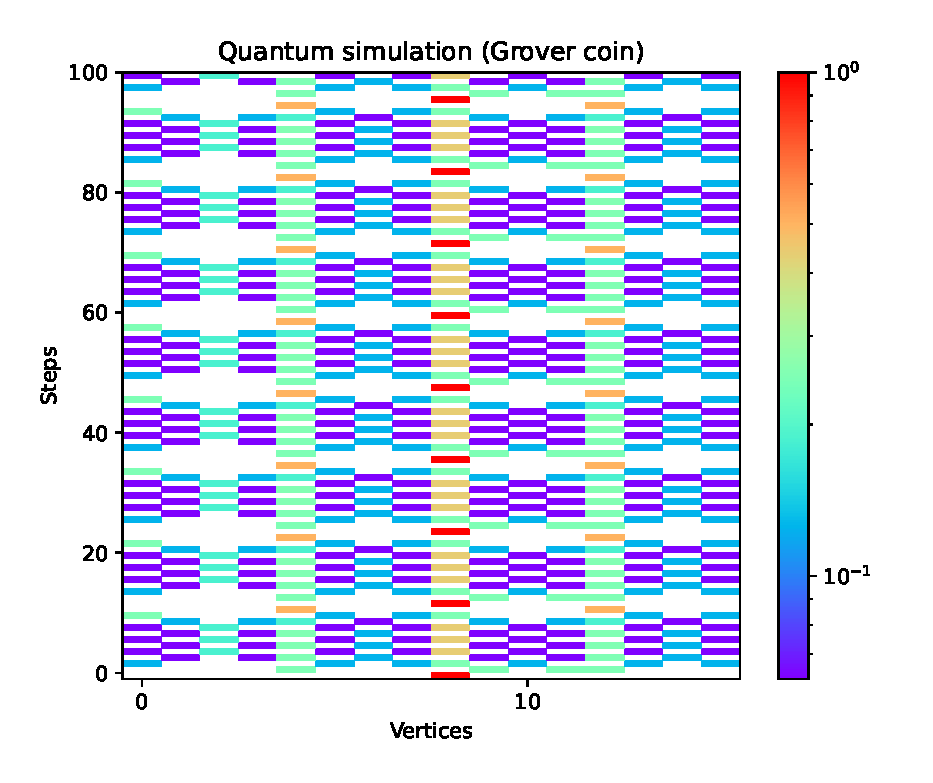
\includegraphics[width=\textwidth]{./figures/results/grid_horizontal_vertical/grover.eps}
    \end{column}
    \begin{column}{.30\textwidth}
      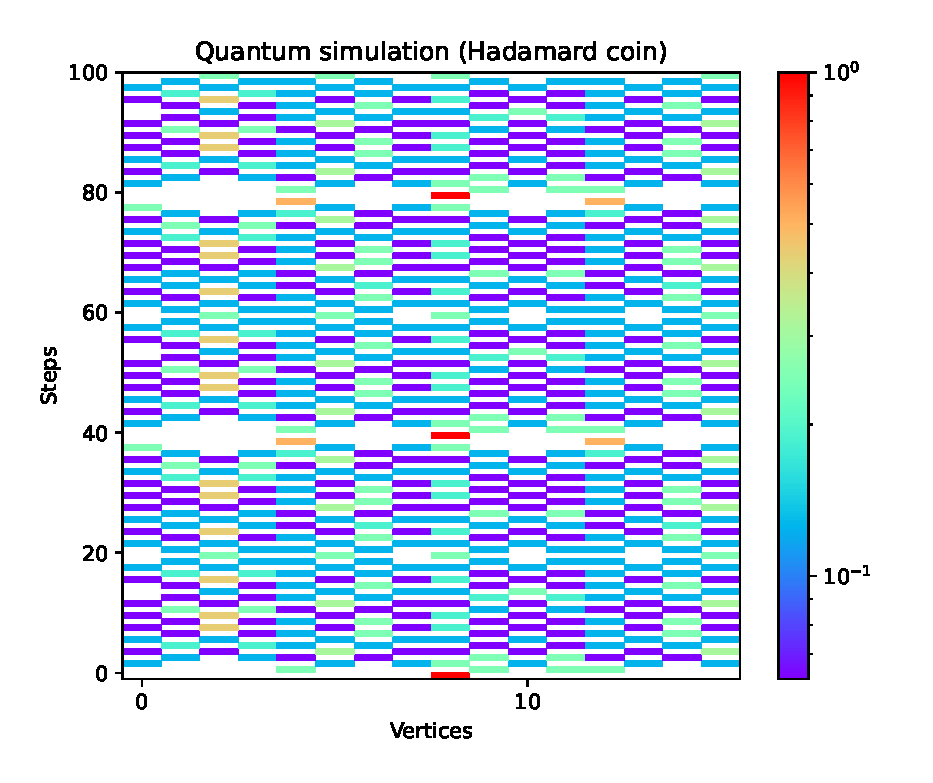
\includegraphics[width=\textwidth]{./figures/results/grid_horizontal_vertical/hadamard.eps}
      \vspace{-1em} % adjust this value as needed
      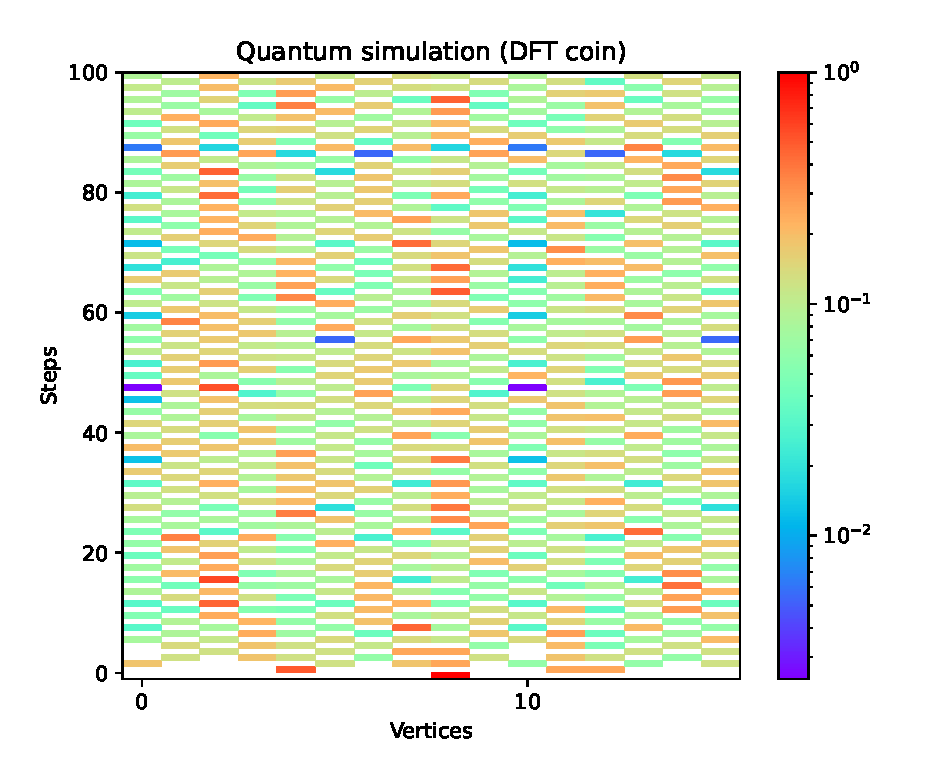
\includegraphics[width=\textwidth]{./figures/results/grid_horizontal_vertical/dft.eps}
    \end{column}
    \begin{column}{.20\textwidth}
    \end{column}
  \end{columns}
\end{frame}


\begin{frame}{Walk in higher dimensions (Hypercube)}
  \begin{columns}[onlytextwidth]
    \begin{column}{.20\textwidth}
    \end{column}
    \begin{column}{.30\textwidth}
      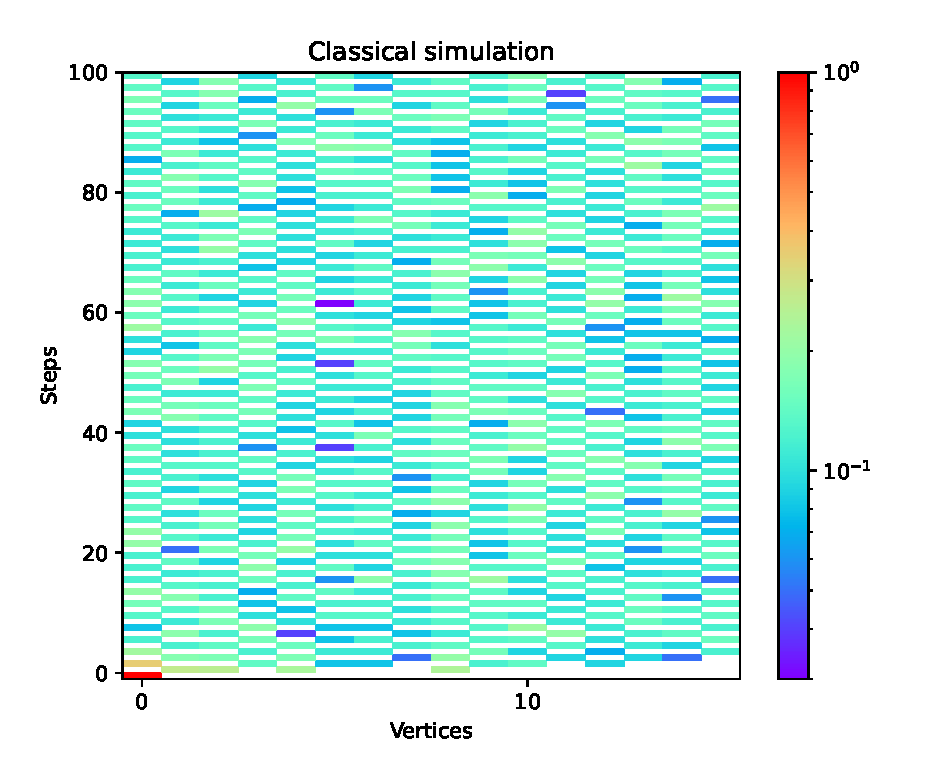
\includegraphics[width=\textwidth]{./figures/results/hypercube/classical.eps}
      \vspace{-1em} % adjust this value as needed
      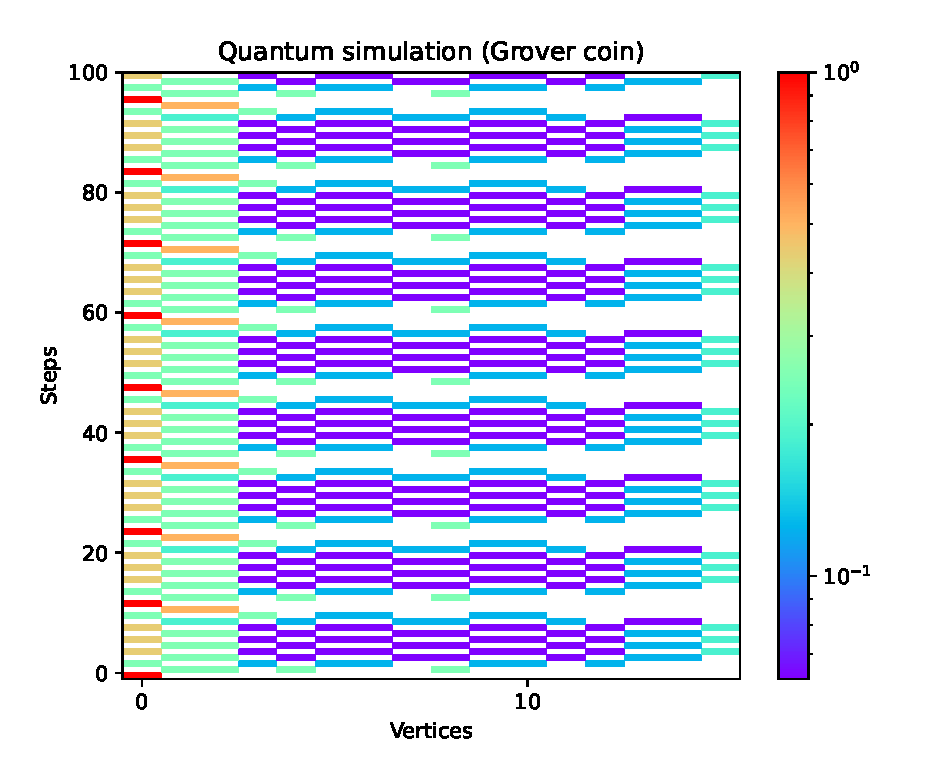
\includegraphics[width=\textwidth]{./figures/results/hypercube/grover.eps}
    \end{column}
    \begin{column}{.30\textwidth}
      \includegraphics[width=\textwidth]{./figures/results/hypercube/hadamard.eps}
      \vspace{-1em} % adjust this value as needed
      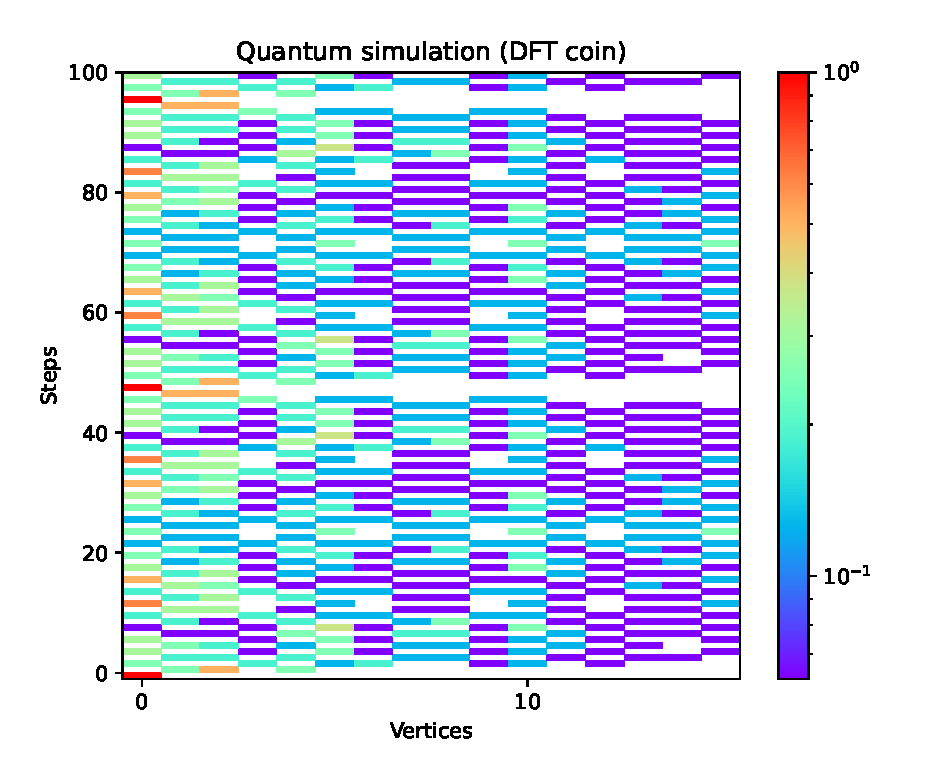
\includegraphics[width=\textwidth]{./figures/results/hypercube/dft.eps}
    \end{column}
    \begin{column}{.20\textwidth}
    \end{column}
  \end{columns}
\end{frame}

\begin{frame}{Current state \& future plans}
\begin{itemize}
    \item 
\end{itemize}
    
\end{frame}

\begin{frame}{Software}
\begin{itemize}
    \item \url{github.com/nemkin/quantum-walk} (open source, MIT license)
\end{itemize}
\end{frame}

\end{document}